\documentclass{beamer}
\usetheme{default} 

\setbeamercolor{structure}{fg=green!40!black} 
\usebackgroundtemplate{
    \centering
\includegraphics[width=\paperwidth,height=\paperheight]{images/android_wall}
}
\setbeamertemplate{navigation symbols}{}

\usepackage[polish]{babel}
\usepackage[utf8x]{inputenc}
\usepackage{t1enc}
\usepackage{default}
\usepackage{listings}

\lstset{language=java, basicstyle=\small, commentstyle=\color{gray}}
\lstset{frame=single}

\usefoottemplate{
  \vbox{
    \tinycolouredline{structure!25}{
      \color{black}\textbf{	
        \insertshortauthor\hfill
        Android @ Szczecin 2011
      } 
    }
%    \tinycolouredline{structure}{
%      \color{white}\textbf{\insertshorttitle}\hfill
%    } 
  }
}

\title{Android @ Szczecin \\ 2011}
\author{Konrad Malawski \\ konrad.malawski@java.pl}

\begin{document}




\begin{frame}
 \begin{center}
  \Huge{Moar* Fun with Views}
 \end{center}
\begin{flushright}
* sic
\end{flushright}
\end{frame}


\begin{frame}\frametitle{Zmierzamy w kierunku kolejnego Activity}
\begin{itemize}
 \item Dodamy nowe Activity
 \pause \item Będzie pobierać coś z sieci (lub udawać) oraz
 \pause \item hint: przyda się jakiś progress bar etc
 \pause \item utworzy z tych danych ListView
 \pause \item przejdziemy do niego przez \textbf{menu} w obecnym Activity
\end{itemize}
\end{frame}

% Menus
\begin{frame}
\begin{center}
 \Huge{Menu}
\end{center}
\end{frame}


\begin{frame}\frametitle{Menu (vide przycisk menu)}
\begin{center}
 Cel:\\
 \begin{figure}
  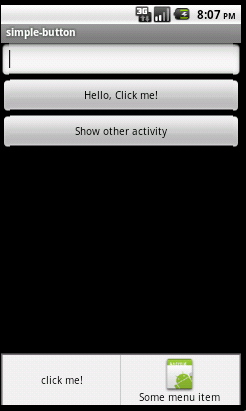
\includegraphics[height=.75\textheight]{images/sample_with_menu}
 \end{figure}
\end{center}
\end{frame}

\begin{frame}[fragile]\frametitle{res/menu/sample\_menu.xml}
\begin{lstlisting}
<menu xmlns:android="http://...">

    <item android:id="@+id/click_me_menu_item"
          android:title="click me!"
            />

    <item android:id="@+id/some_menu_item"
          android:title="Some menu item"
          android:icon="@drawable/icon"
            />
</menu>
\end{lstlisting}
\end{frame}

\begin{frame}[fragile]\frametitle{SomeActivity\#onCreateOptionsMenu}
\begin{lstlisting}
@Override
public boolean onCreateOptionsMenu(Menu menu) { 
  MenuInflater inflater = getMenuInflater();

  inflater.inflate(R.menu.sample_menu, menu);
  return true;
}
\end{lstlisting}
\end{frame}

\begin{frame}[fragile]\frametitle{SomeActivity\#onCreateOptionsMenu}
\begin{lstlisting}
@Override
public boolean onCreateOptionsMenu(Menu menu) { 
  MenuInflater inflater = getMenuInflater();

  inflater.inflate(R.menu.sample_menu, menu);
  return true; // true == ma zostac pokazane
}
\end{lstlisting}
\end{frame}

\begin{frame}[fragile]\frametitle{SomeActivity\#onOptionsItemSelected}
\begin{lstlisting}
@Override
public boolean onOptionsItemSelected(MenuItem item) {
  int itemId = item.getItemId();

  switch (itemId){
    case R.id.click_me_menu_item:
      doSomething();
      break;
    default:
      Log.i(TAG, "Some weird action was requested");
  }

  return true; 
}
\end{lstlisting}
\end{frame}

\begin{frame}[fragile]\frametitle{SomeActivity\#onOptionsItemSelected}
\begin{lstlisting}
@Override
public boolean onOptionsItemSelected(MenuItem item) {
  int itemId = item.getItemId();

  switch (itemId){
    case R.id.click_me_menu_item:
      doSomething();
      break;
    default:
      Log.i(TAG, "Some weird action was requested");
      return false;
  }

  return true; // true == obsluzylismy event
               //      == no need to bubble it
}
\end{lstlisting}
\end{frame}


% MORE FUN UI STUFF
\begin{frame}
\begin{center}
 \Huge{Giving Feedback} \\
 \large{(Toasts and Dialogs)}
\end{center}
\end{frame}


\begin{frame}[fragile]\frametitle{Pyszne tosty z masełkiem (android.widget.Toast)}

\begin{figure}[h]
 \centering
 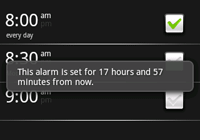
\includegraphics[height=0.40\textheight,keepaspectratio=true]{images/toast}
\end{figure}

 Przykład użycia: 
 \begin{lstlisting}
Toast.makeText(getApplicationContext(),
               "Halo Szczecin!", 
               Toast.LENGTH_LONG)
     .show();
 \end{lstlisting}

\end{frame}

\begin{frame}[fragile]
\frametitle{Co więcej potrafi Toast?}
\begin{lstlisting}
 Toast t = Toast.makeText(this, txt, LENGTH_SHORT);
\end{lstlisting}

\pause

Można mu zmienić pozycję:
\begin{lstlisting}
t.setGravity(Gravity.TOP|Gravity.LEFT, 0, 0);
\end{lstlisting}

\pause

lub podmienić widok:
\begin{lstlisting}
View customView = findViewById(R.id.custom_view);
/**/
t.setView(customView)
 \end{lstlisting}

\end{frame}

\begin{frame}
 \begin{center}
  \Huge{Dialog}
 \end{center}
\end{frame}


\begin{frame}\frametitle{Dialog - wyskakuje 'nad' Activity}
\begin{columns}
 \column{.5\textwidth}
  \begin{figure}
   \centering
   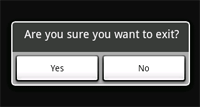
\includegraphics[width=.7\textwidth]{images/dialog_buttons}
  \end{figure}
  \begin{figure}
   \centering
   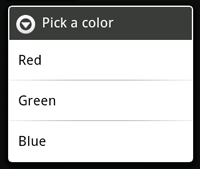
\includegraphics[width=.7\textwidth]{images/dialog_list}
  \end{figure}
 \column{.5\textwidth}
 \begin{figure}
   \centering
   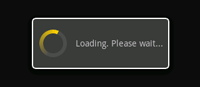
\includegraphics[width=.7\textwidth]{images/dialog_progress_spinning}
  \end{figure}
  \begin{figure}
   \centering
   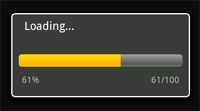
\includegraphics[width=.7\textwidth]{images/dialog_progress_bar}
  \end{figure}
\end{columns}
\end{frame}

% \begin{frame}[fragile]\frametitle{List Dialog}
% \begin{lstlisting}
% final CharSequence[] items = {"Red", "Green", "Blue"};
% 
% AlertDialog.Builder builder = new AlertDialog.Builder(this);
% builder.setTitle("Pick a color");
% builder.setItems(items, new DialogInterface.OnClickListener() {
%  public void onClick(DialogInterface dialog, int item) {
%   Toast.makeText(getApplicationContext(), items[item], Toast.LENGTH_SHORT).show();
%  }
% });
% AlertDialog alert = builder.create();
% \end{lstlisting}
% \end{frame}

\begin{frame}[fragile]\frametitle{Progress Dialog (Spinning)}
\begin{lstlisting}
ProgressDialog dialog = ProgressDialog
                           .show(MyActivity.this, 
                                 "", 
                                 "Loading. Please wait...", 
                                 true);
\end{lstlisting}

\begin{figure}
 \centering
 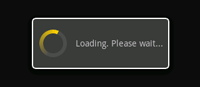
\includegraphics[width=.5\textwidth]{images/dialog_progress_spinning}
\end{figure}

\pause

\begin{lstlisting}
dialog.hide();
\end{lstlisting}
\end{frame}

\begin{frame}[fragile]\frametitle{Super Fast Java Reminder - \textbf{this}}
Pamiętamy dlaczego w poprzednim przykładzie powinno (często) być \textbf{MyActivity.this}?
\begin{lstlisting}
class Outer extends Activity { 

  void onCreate(Bundle savedState) {

    new OnClickListener() {
      public void onClick(View view) {
        new Intent(this, /*...*/); // ZLE!
      }
    }

  }
}
\end{lstlisting}
\end{frame}

\begin{frame}[fragile]\frametitle{Super Fast Java Reminder - \textbf{this}}
Oto jak dobrać się do ,,zewnętrznego'' \textbf{this}:
\begin{lstlisting}
class Outer extends Activity { 

  void onCreate(Bundle savedState) {

    new OnClickListener() {
      public void onClick(View view) {
        new Intent(Outer.this, /*...*/); // Dobrze
      }
    }

  }
}
\end{lstlisting}
\end{frame}







\end{document}
